\documentclass[a4paper]{jarticle}
\usepackage{tani_resume}
\usepackage{epstopdf}
\usepackage{graphicx}
\usepackage{ascmac}
\alignbeforeskip -5mm
\alignafterskip -5mm
\eqnarraybeforeskip -5mm
\eqnarrayafterskip -5mm
\makeatletter
\newenvironment{figurehere}
  {\def\@captype{figure}}
  {}
\makeatother

\jptitle{国際情報科学コンテスト 『ビーバーコンテスト 』\\国内コンテストページの試作}
\etitle{}
\jpauthor{鈴木一至 佐々木陽広}
\eauthor{Kazushi Suzuki,Akihiro Sasaki}
\course{谷聖一研究室}
\year{27}


%% 概要 %%
\abstract{

コンピュータ・サイエンスの普及を目的とした取り組みは,様々なところで行われている.
その中の1つに,小・中・高校生を対象にした「ビーバーコンテスト」がある.フランスのグループがビーバーコンテストのサーバシステムを開発し,オープンソースとして公開している.本演習では,このサーバシステムを元に,事後学習として過去に行われたビーバーコンテストにチャレンジできるWebページを試作した.}
\compheading

\begin{document}
\maketitle
\begin{multicols}{2}
\setcounter{page}{1}

\section{はじめに}

\subsection{ビーバーコンテストとは}
\subsubsection{概要}
ビーバーコンテスト(\cite{bebras-contest, bebras-pdf})とは,2004年にリトアニアで始められた国際的な情報科学コンテストである.日本の小学5年生から高等学校3年生を対象とし、年に1回開催される.日本は2011年度から正式参加しており,2014年には世界35カ国から92万人の児童・生徒が参加している.情報科学の事前知識がなくても解くことが可能な問題を扱い,問題に取り組むことによって情報科学の基礎概念に触れることができ,論理的思考の向上の一助になるようなものになっている.また,コンテスト後に参加者同士で問題の内容について議論することで,情報科学に興味を持つきっかけになることが期待される.

\subsubsection{形式}
 コンテストの問題は年齢に応じた区分ごとに用意されており,基本はベンジャミン(小学5年生・6年生),カデット(中学1年生・2年生),ジュニア(中学3年生・高校1年生),シニア(高校2年生・3年生)の4区分であり,日本ではベンジャミンが30分10問,その他が40分12問で実地している.
\\ 問題形式は大きく2種類あり,動的にオブジェクトを操作しながら試行錯誤できる対話型と,それに対する非対話型がある.また,非対話型の中には選択肢を選んで解く選択肢型と,文字を入力して解答する文字入力型がある.

\subsection{目的}
現在,ビーバーコンテストを受けるには離れたオランダのサーバに接続する必要があり、コンテストを受ける環境によっては正常に問題を受けることができない場合があった.この問題を解消するために,手元の環境で試作し,主に日本から過去のコンテストを受ける際に正常に動作できるWebページを試作することが本演習の目的である.
また,来年以降の展望として,過去のコンテストだけでなく,年1回行われる正式なコンテストも受験可能になることがあげられる.

\section{準備}

\subsection{用語説明}
\begin{description}
\item[Git]プログラムのソースコードなどの変更履歴を記録・追跡するための分散型バージョン管理システムである.また,Gitを使用してソフトウェア開発プロジェクトのための共有ウェブサービスとしてGIthubがある.(詳細は\cite{git}参照)
\end{description}

\begin{description}
\item[Bower]Twitter社によるフロントエンド用パッケージ管理ツールである.json形式の設定ファイルを用意することで,記述されたパッケージを一括で取り込むことができる.(詳細は\cite{bower}参照)
\end{description}

\begin{description}
\item[Composer] PHPの依存関係管理ツールである.bowerと同じくjsonから複数のパッケージをインストールすることができる.(詳細は\cite{composer}参照)

\end{description}

\begin{description}
\item[DBV]  Webページ上でデータベース管理を行うためのツールである.(詳細は\cite{dbv}参照)
\end{description}

\begin{description}
\item[i18n] 国際化を意味するinternationalizationを省略した記述法で表したものである.国際化とは「ソフトウェアに技術的な変更を加えることなく多様な言語や地域に適合できるようにする,ソフトウェア設計の工程である」(\cite{i18n}).
\end{description}

\subsection{試作環境}
\begin{itemize}
\item 仮想サーバ:VMware
\item CPU:1個
\item OS:Ubuntu Linux (64bit)
\item Apache + MySQL + PHP
\end{itemize}

\section{試作手順}
本演習では,事後学習として過去に行われたビーバーコンテストにチャレンジできるWebページを試作した.報告者は,フランスのグループがGithubに公開しているサーバシステム(\cite{bebras-france-platform})を元に開発を進めた.本章では,報告者が試作した手順を記す.
\subsection{オープンソースのインストール}
Gitを用いて,フランスのグループがGithubに公開しているサーバシステム(\cite{bebras-france-platform})を入手した.しかし,このサーバーシステムはまだ未完全であったこともあり,Github上での更新を確認しつつ進めていく形となった.

\subsection{パッケージのインストール}
今回試作するサーバーシステムにはフロントエンドとPHPそれぞれのパッケージを導入する必要があった.本演習では,フロントエンド用にbower,PHP用にcomposerを使用し,それぞれが必要な内容が記述されたjsonファイルを元にパッケージの取り込みを行った.

\subsection{データベース構築}
dbvを用いることで,ブラウザを通してデータベースを作成した.元となるsql文はテーブルごとにフォルダに格納されており,dbvはそのフォルダ内のファイルを一括で実行することができる.

\subsection{翻訳}
ページの言語には,英語が使われており,そのままでは日本の学生が使うことは困難であるため,翻訳が必要であった.そこで「i18next」というフロントエンドで国際化を可能にするライブラリを用いて翻訳を行った.以下,具体的な使用法の説明をする.HTML内では,data-i18n属性を用い,それぞれ翻訳箇所に任意の文字列を当てる(図\ref{fig:101}参照).

\begin{figurehere}
\begin{center}
\fbox{
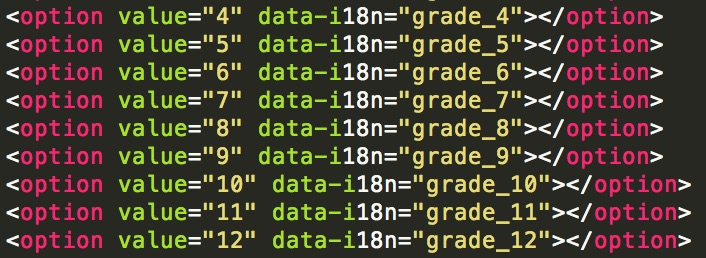
\includegraphics[bb=0 0 706 258,width=7.5cm]{img/i18n_1.jpg}
}
\end{center}
\caption{翻訳時のHTML内の記述}\label{fig:101}
\end{figurehere}

翻訳箇所に当てられた文字列をリストでまとめているjsonファイルを用いて,翻訳を行う.左側の文字列に対応する翻訳した文字列を右に入力することで(図\ref{fig:102},図\ref{fig:103}参照),ページ上には翻訳された文字が表示できるようになる.また言語のフォルダごとにjsonファイルを作り,記述しておくことで容易に国際化が可能となる.

\begin{figurehere}
\begin{center}
\fbox{
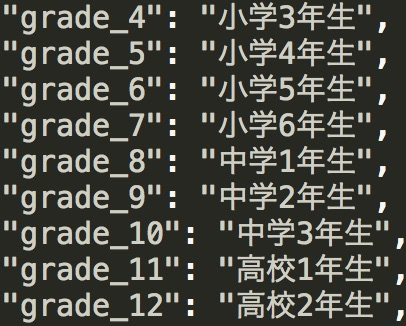
\includegraphics[bb=0 0 406 326,width=5.8cm]{img/i18n_ja.jpg}
}
\end{center}
\caption{jsonファイル内の記述(日本語化の場合)}\label{fig:102}
\end{figurehere}

\begin{figurehere}
\begin{center}
\fbox{
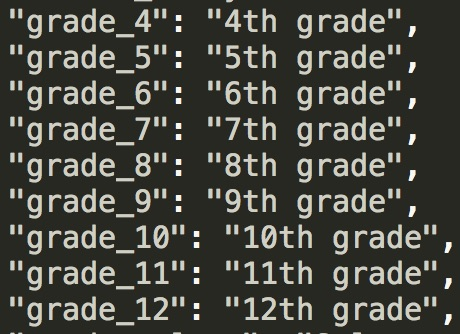
\includegraphics[bb=0 0 460 334,width=6cm]{img/i18n_en.jpg}
}
\end{center}
\caption{jsonファイル内の記述(英語化の場合)}\label{fig:103}
\end{figurehere}


\section{ビーバーコンテストページの試作}
本項では,報告者が試作した過去のコンテストまたは,新規コンテストを受験することができる「ビーバーコンテストページ」の機能について述べる.

\subsection{コンテスト選択画面}
今回試作したWebページのトップにあたるコンテスト選択画面では,「新規コンテストの受験」「過去のコンテストの受験」「受験したコンテストの結果参照」を選択できる.

\begin{figurehere}
\begin{center}
\fbox{
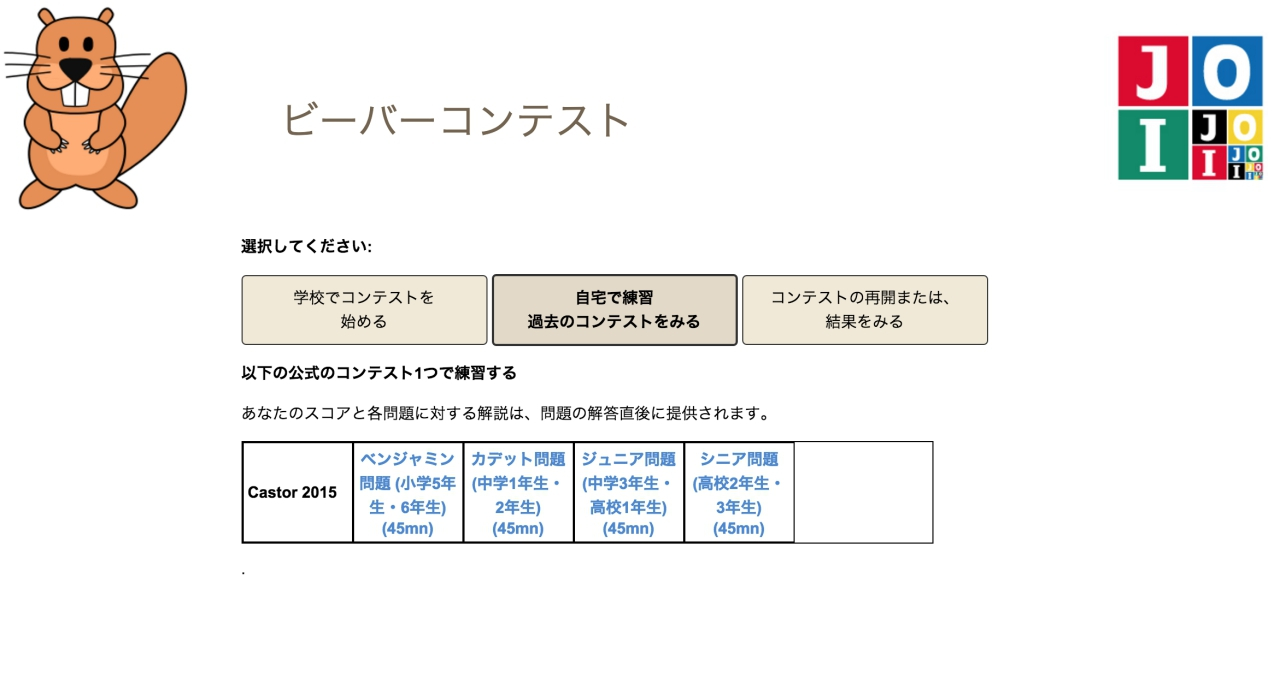
\includegraphics[bb=0 0 1280 679,width=8cm]{img/bebras_top.jpg}
}
\end{center}
\caption{試作したビーバーコンテストのトップページ}\label{fig:1}
\end{figurehere}

\subsection{コンテスト受験}
\subsubsection{過去のコンテスト}
過去のコンテストを選択すると,アクセスコードが表示され,書き留めてからコンテストを開始するよう促される(図\ref{fig:2}参照).アクセスコードとは,コンテスト受験者一人ひとりに提供される一意の文字列である.アクセスコードが提供されることにより,コンテスト時間内に中断したコンテストの再開が可能になったり,受験後に結果を参照することができる.

\begin{figurehere}
\begin{center}
\fbox{
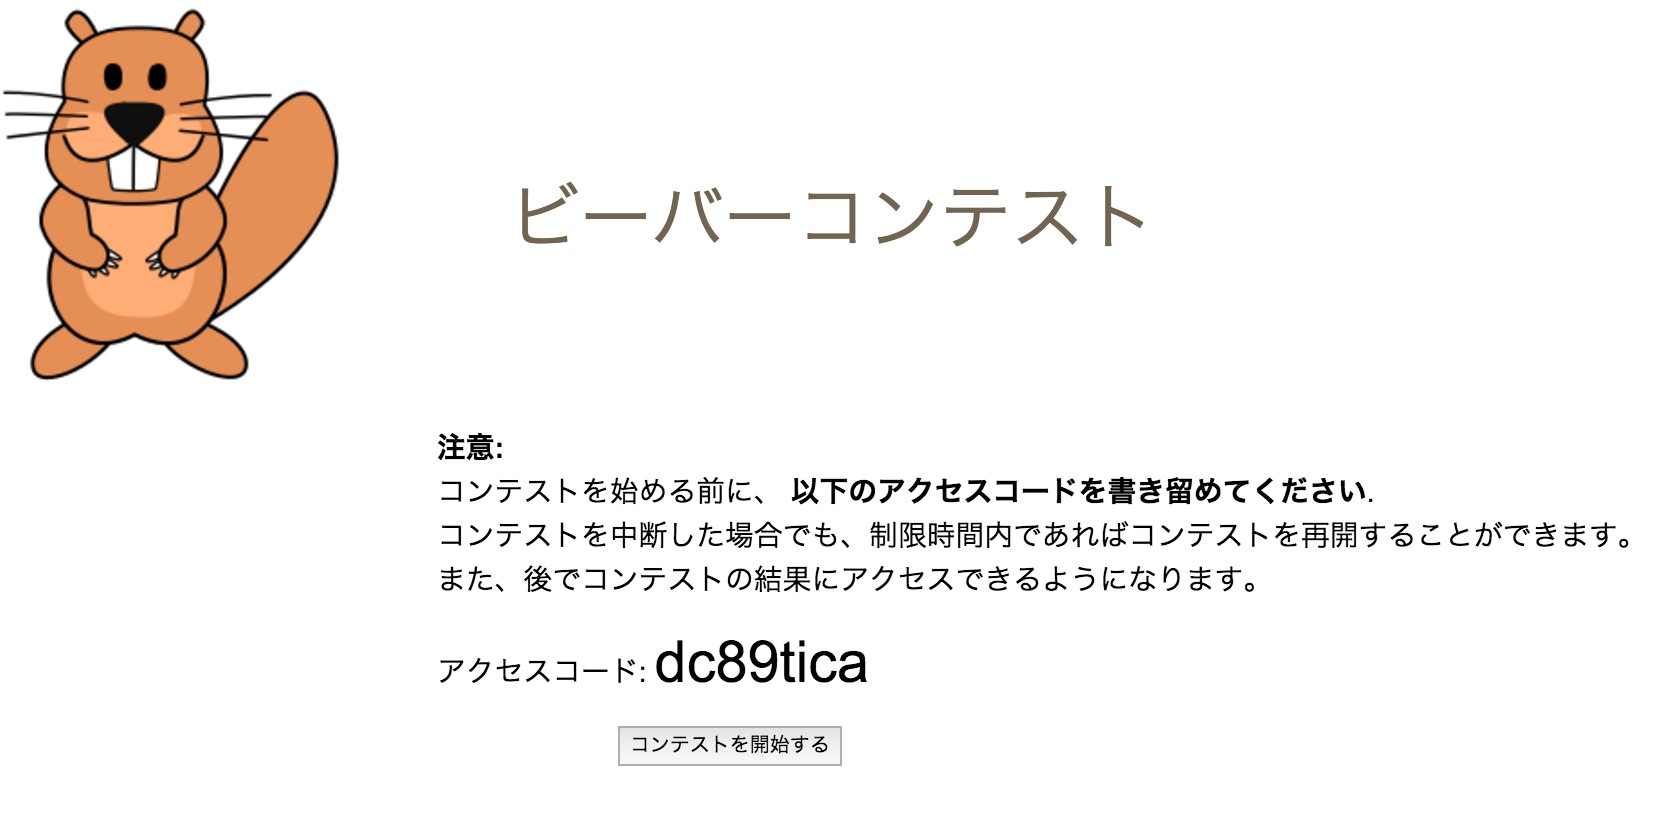
\includegraphics[bb=0 0 1678 826,width=7.5cm]{img/contest_access.jpg}
}
\end{center}
\caption{コンテストのアクセスコード提供}\label{fig:2}
\end{figurehere}

アクセスコードを控え,コンテストの開始ボタンをクリックするとコンテストがロードされる(図\ref{fig:3}参照).受験者は問題を選択し,それぞれの解答を入力する.過去のコンテストでは,全ての問題を解き終えたら,終了ボタンを押すことで問題の解答を確認することができる(図\ref{fig:4}参照).また,解答を入力した瞬間に正誤評価され,リアルタイムで結果を見ながら問題を解くことができる.


\begin{figurehere}
\begin{center}
\fbox{
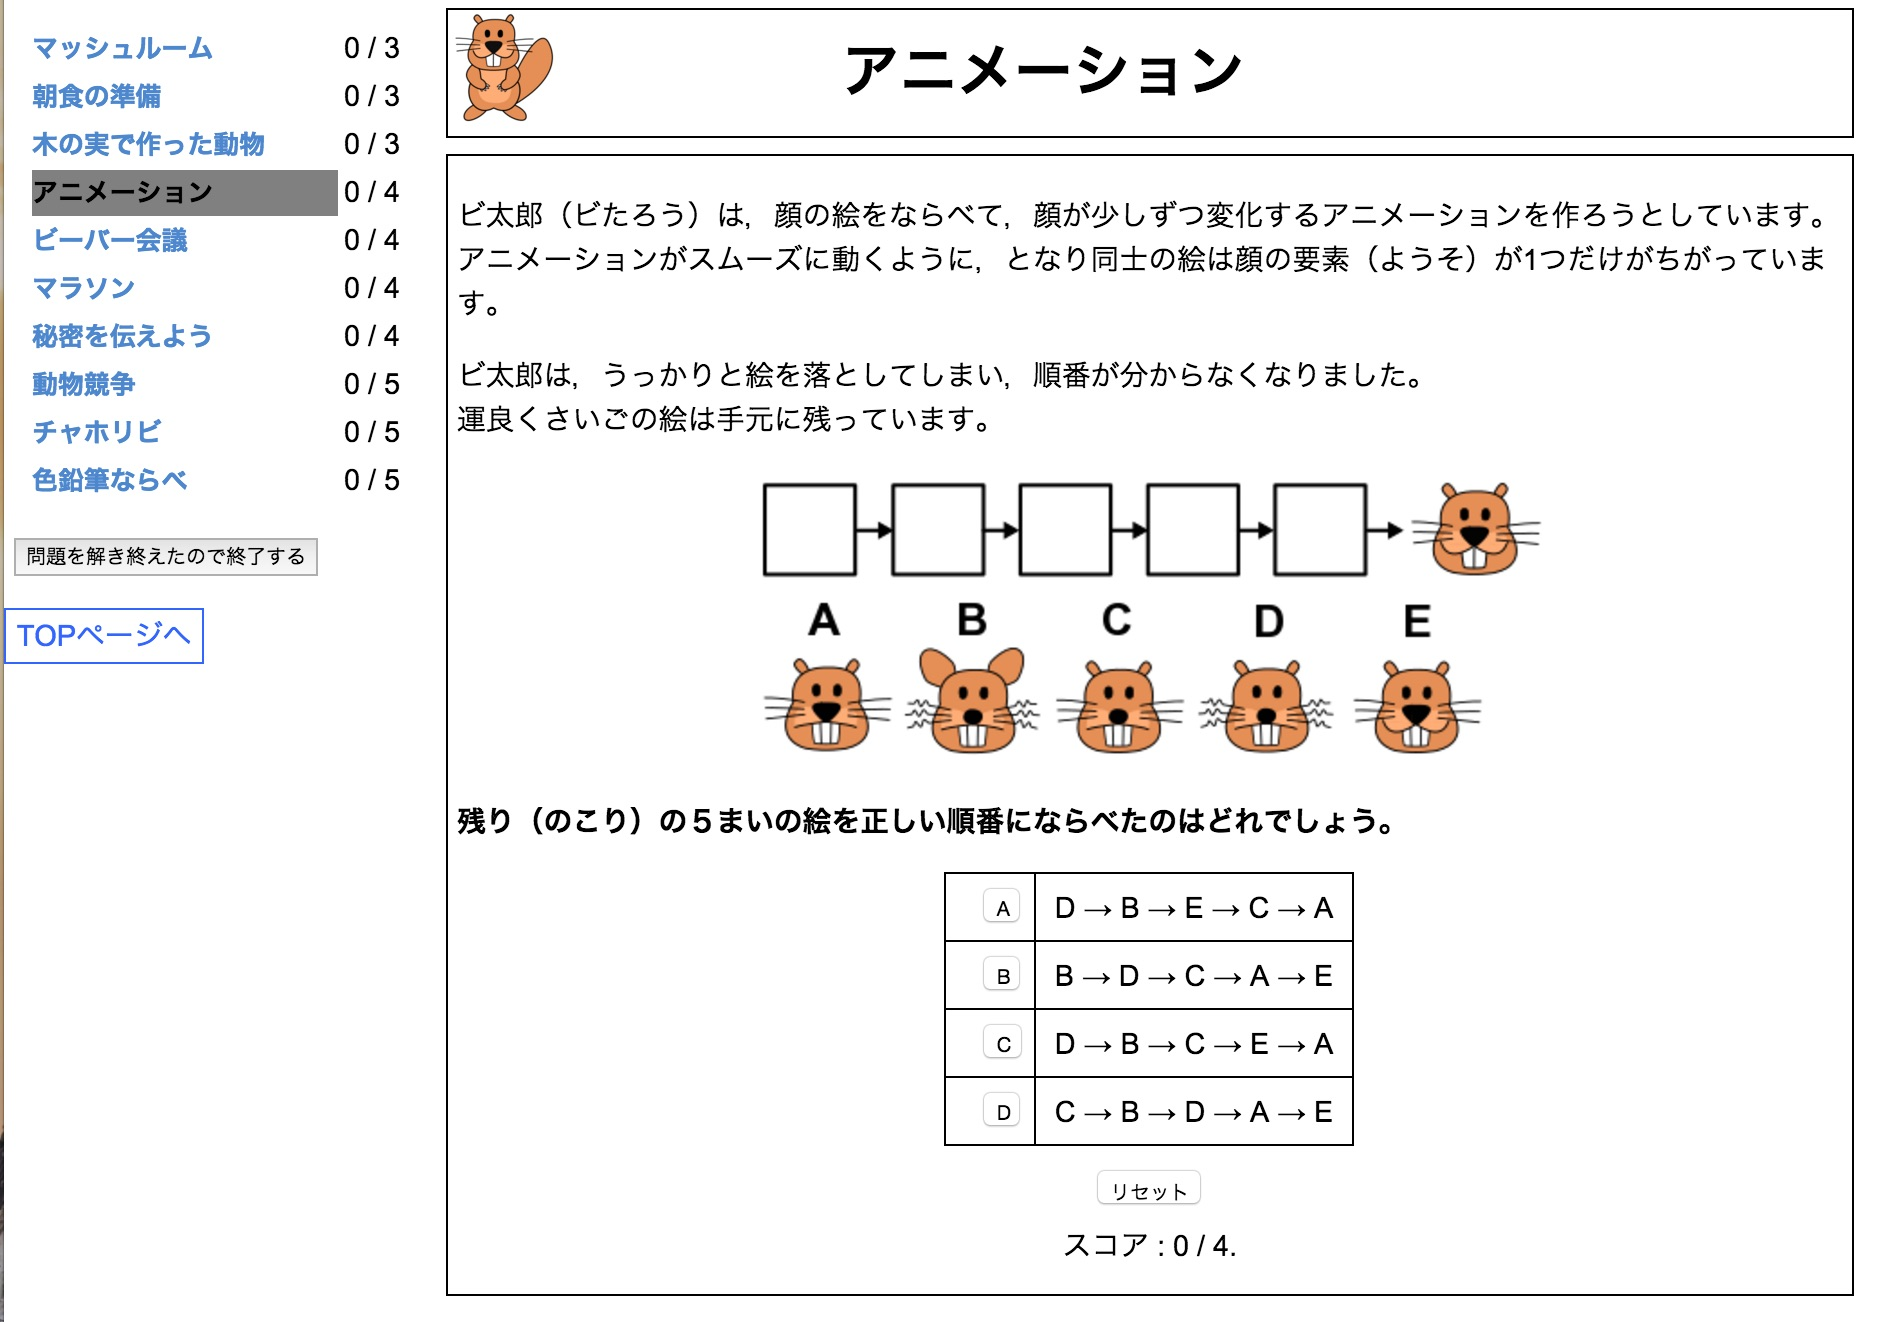
\includegraphics[bb=0 0 1894 1322,width=7.5cm]{img/past_contest_1.jpg}
}
\end{center}
\caption{過去のコンテスト受験}\label{fig:3}
\end{figurehere}

\begin{figurehere}
\begin{center}
\fbox{
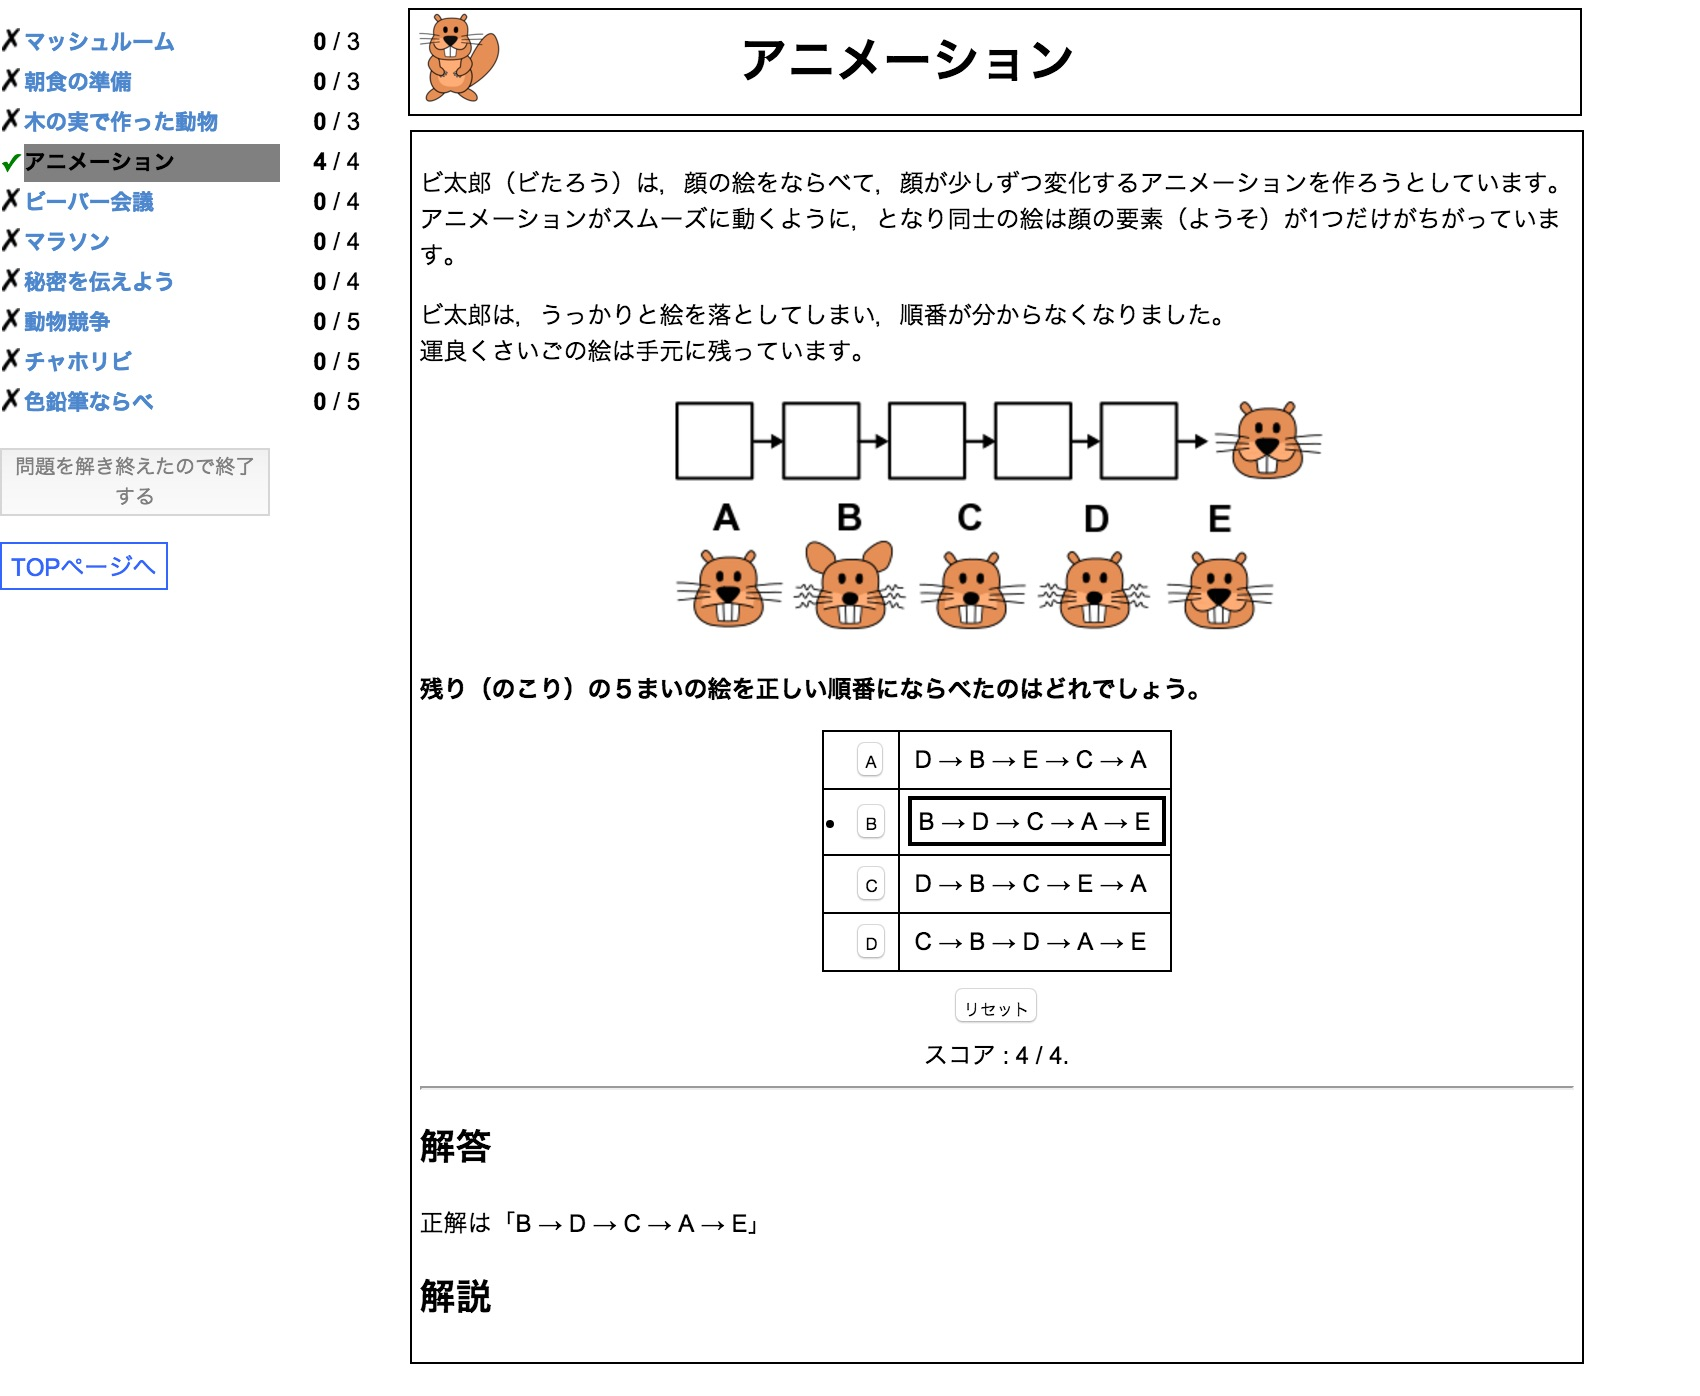
\includegraphics[bb=0 0 1700 1396,width=7.5cm]{img/past_contest_2.jpg}
}
\end{center}
\caption{過去のコンテスト解答確認}\label{fig:4}
\end{figurehere}

\subsubsection{新規コンテスト}
新規コンテストの受験は,教師などから提供されたグループコードを入力することにより,過去のコンテストと同様にアクセスコードが提供され(図\ref{fig:2}参照),コンテストを開始することができる.

\begin{figurehere}
\begin{center}
\fbox{
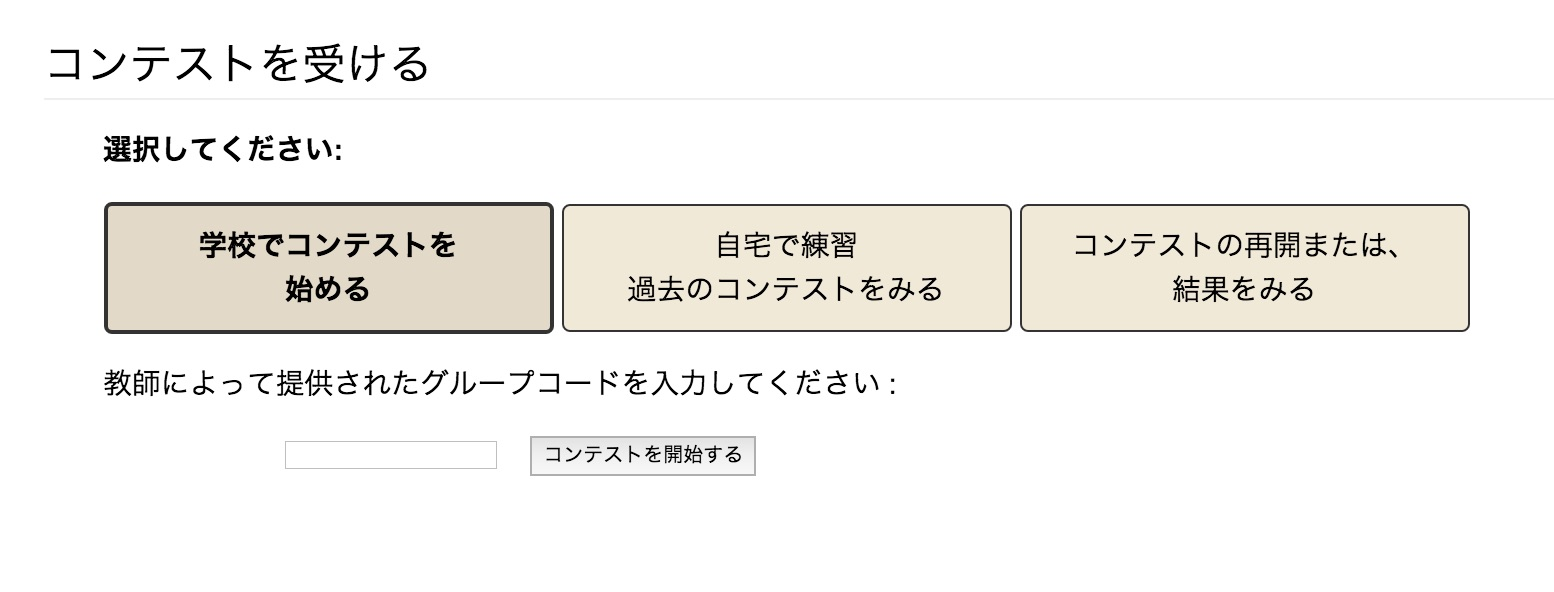
\includegraphics[bb=0 0 1554 592,width=7.5cm]{img/new_contest_start.jpg}
}
\end{center}
\caption{新規コンテスト開始時}\label{fig:5}
\end{figurehere}

新規コンテストでは,過去のコンテストと違い,リアルタイムで結果を見ながら解くことができない仕様となっている(図\ref{fig:6}参照).また,解答後,終了ボタンを押すと図7のメッセージが表示され,問題の解答を確認することができない.これは,1年に1回行われるビーバーコンテストに対応した仕様であり,コンテスト期間中は解答の結果参照が不可となるものである.

\begin{figurehere}
\begin{center}
\fbox{
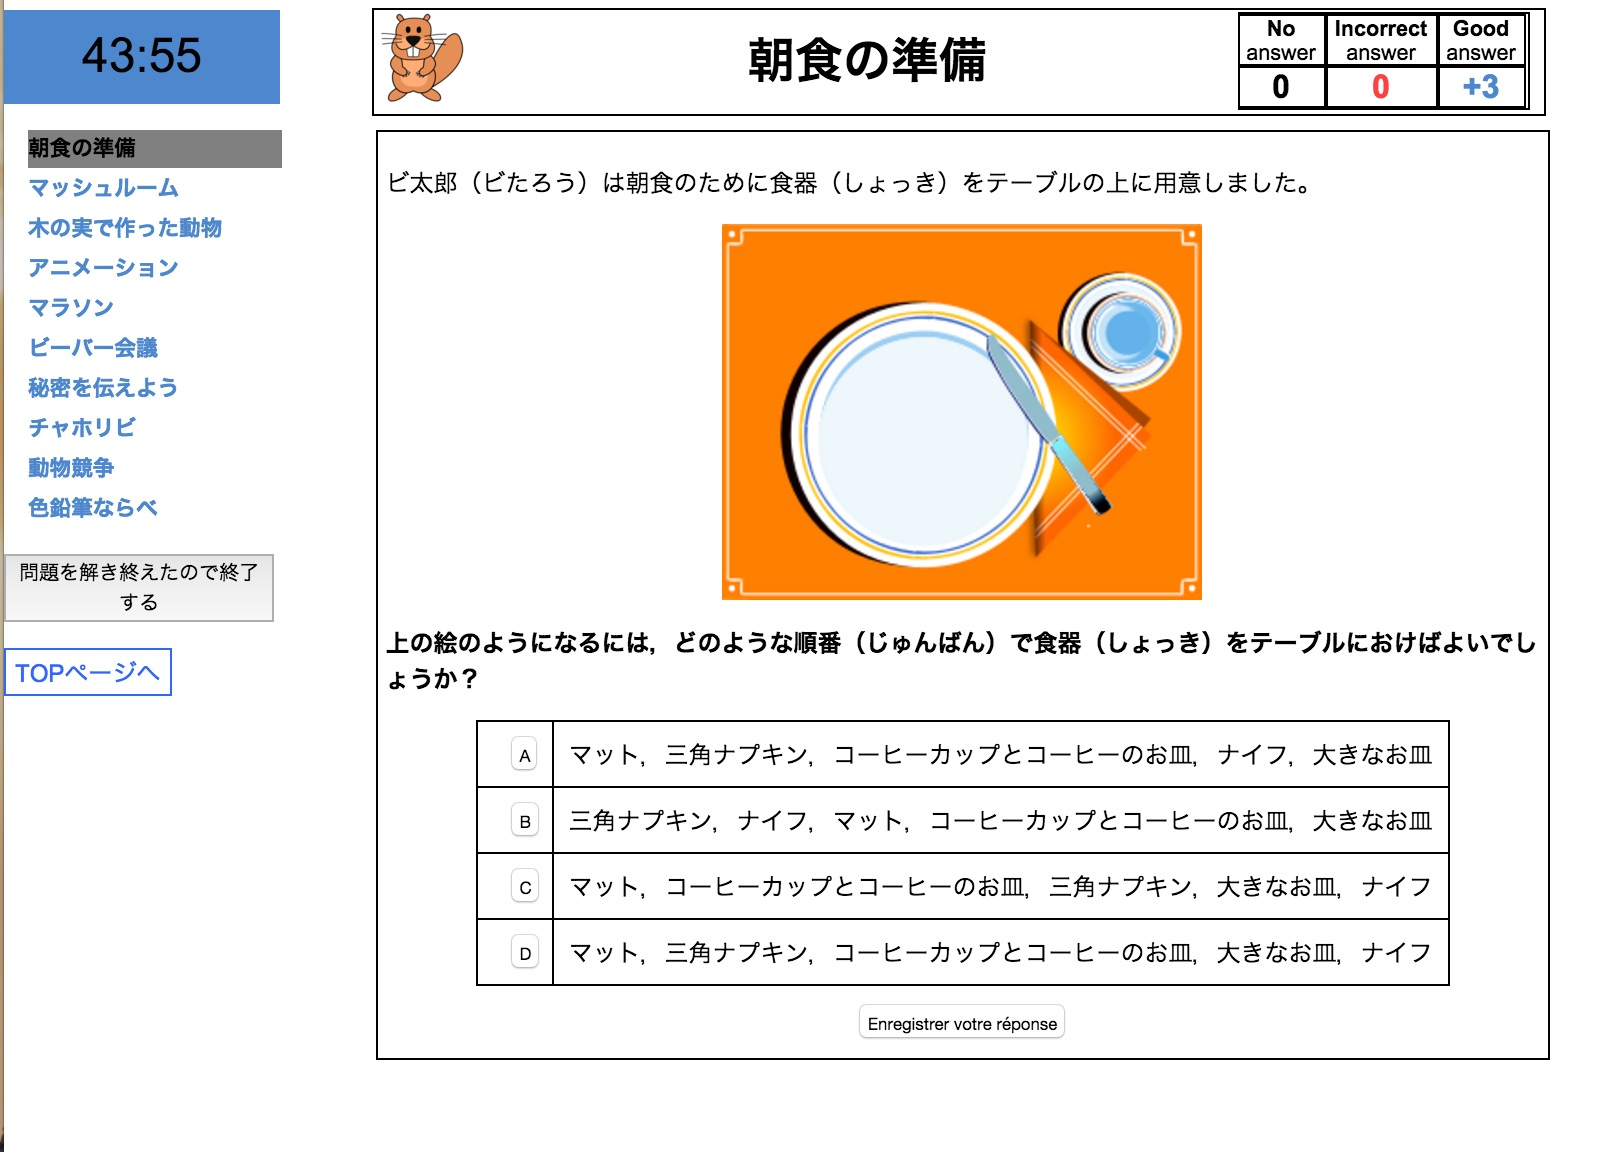
\includegraphics[bb=0 0 1610 1152,width=7.5cm]{img/new_contest_1.jpg}
}
\end{center}
\caption{新規コンテスト受験}\label{fig:6}
\end{figurehere}

\begin{figurehere}
\begin{center}
\fbox{
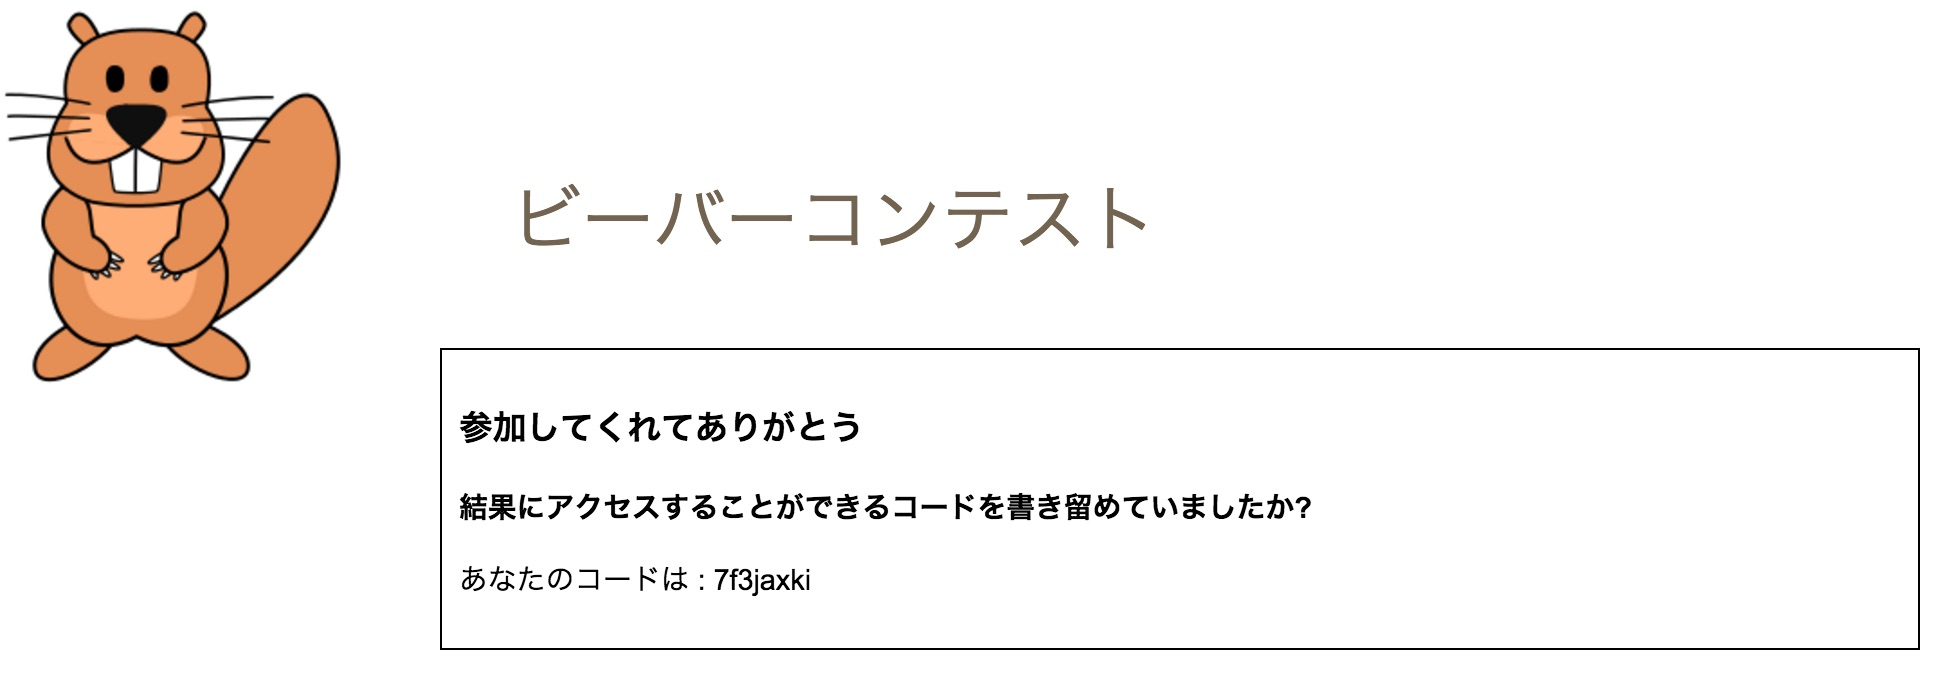
\includegraphics[bb=0 0 1960 696,width=7.5cm]{img/contest_end.jpg}
}
\end{center}
\caption{新規コンテスト受験後}\label{fig:7}
\end{figurehere}


\subsection{コンテスト結果の参照}

新規コンテストの受験者はコンテスト期間を過ぎた後,コンテスト開始時に提供されたアクセスコードを用いて,結果にアクセスすることができる(図\ref{fig:8},図\ref{fig:9}参照).

\begin{figurehere}
\begin{center}
\fbox{
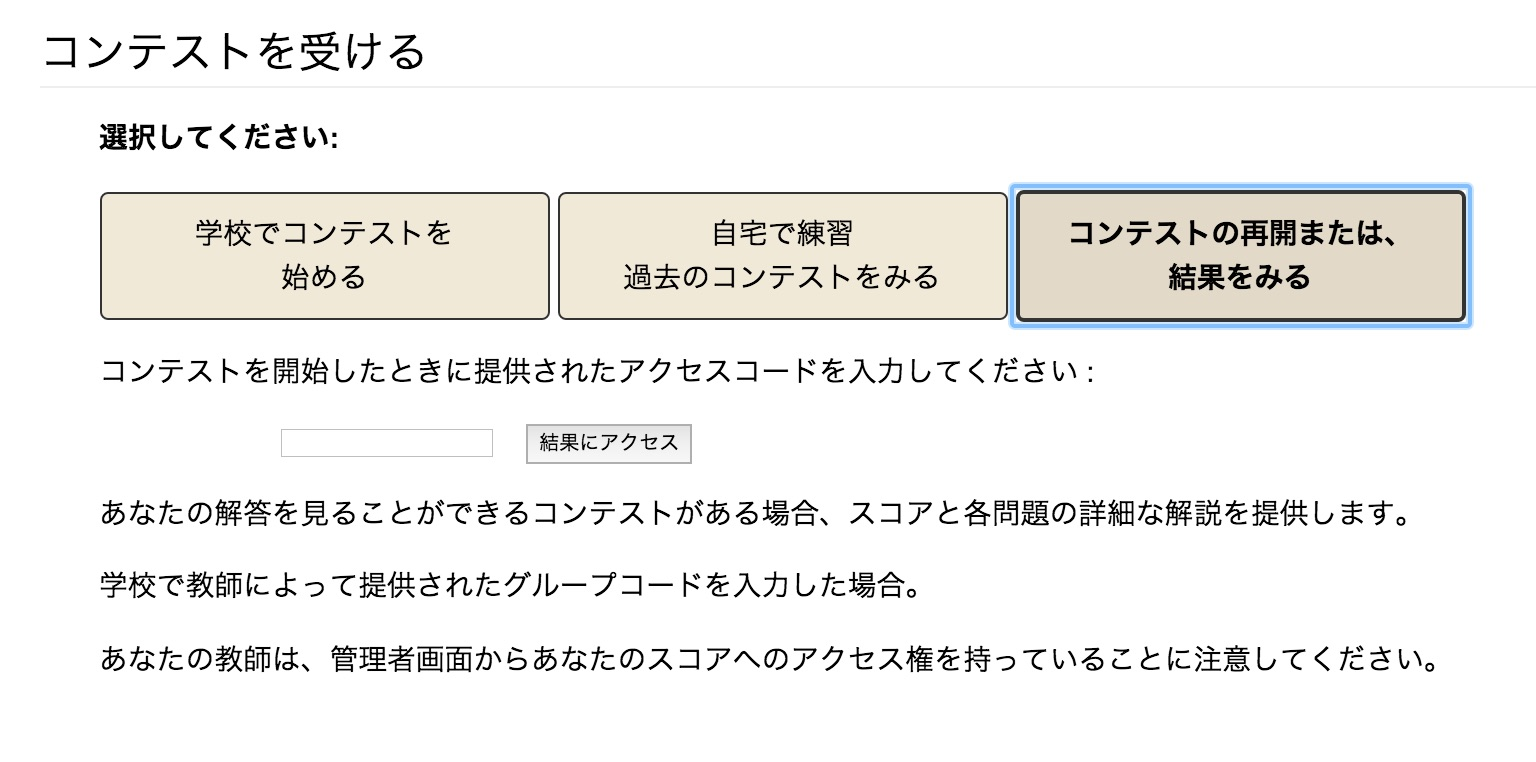
\includegraphics[bb=0 0 1536 762,width=7.5cm]{img/contest_result.jpg}
}
\end{center}
\caption{コンテストの結果へアクセス}\label{fig:8}
\end{figurehere}


\begin{figurehere}
\begin{center}
\fbox{
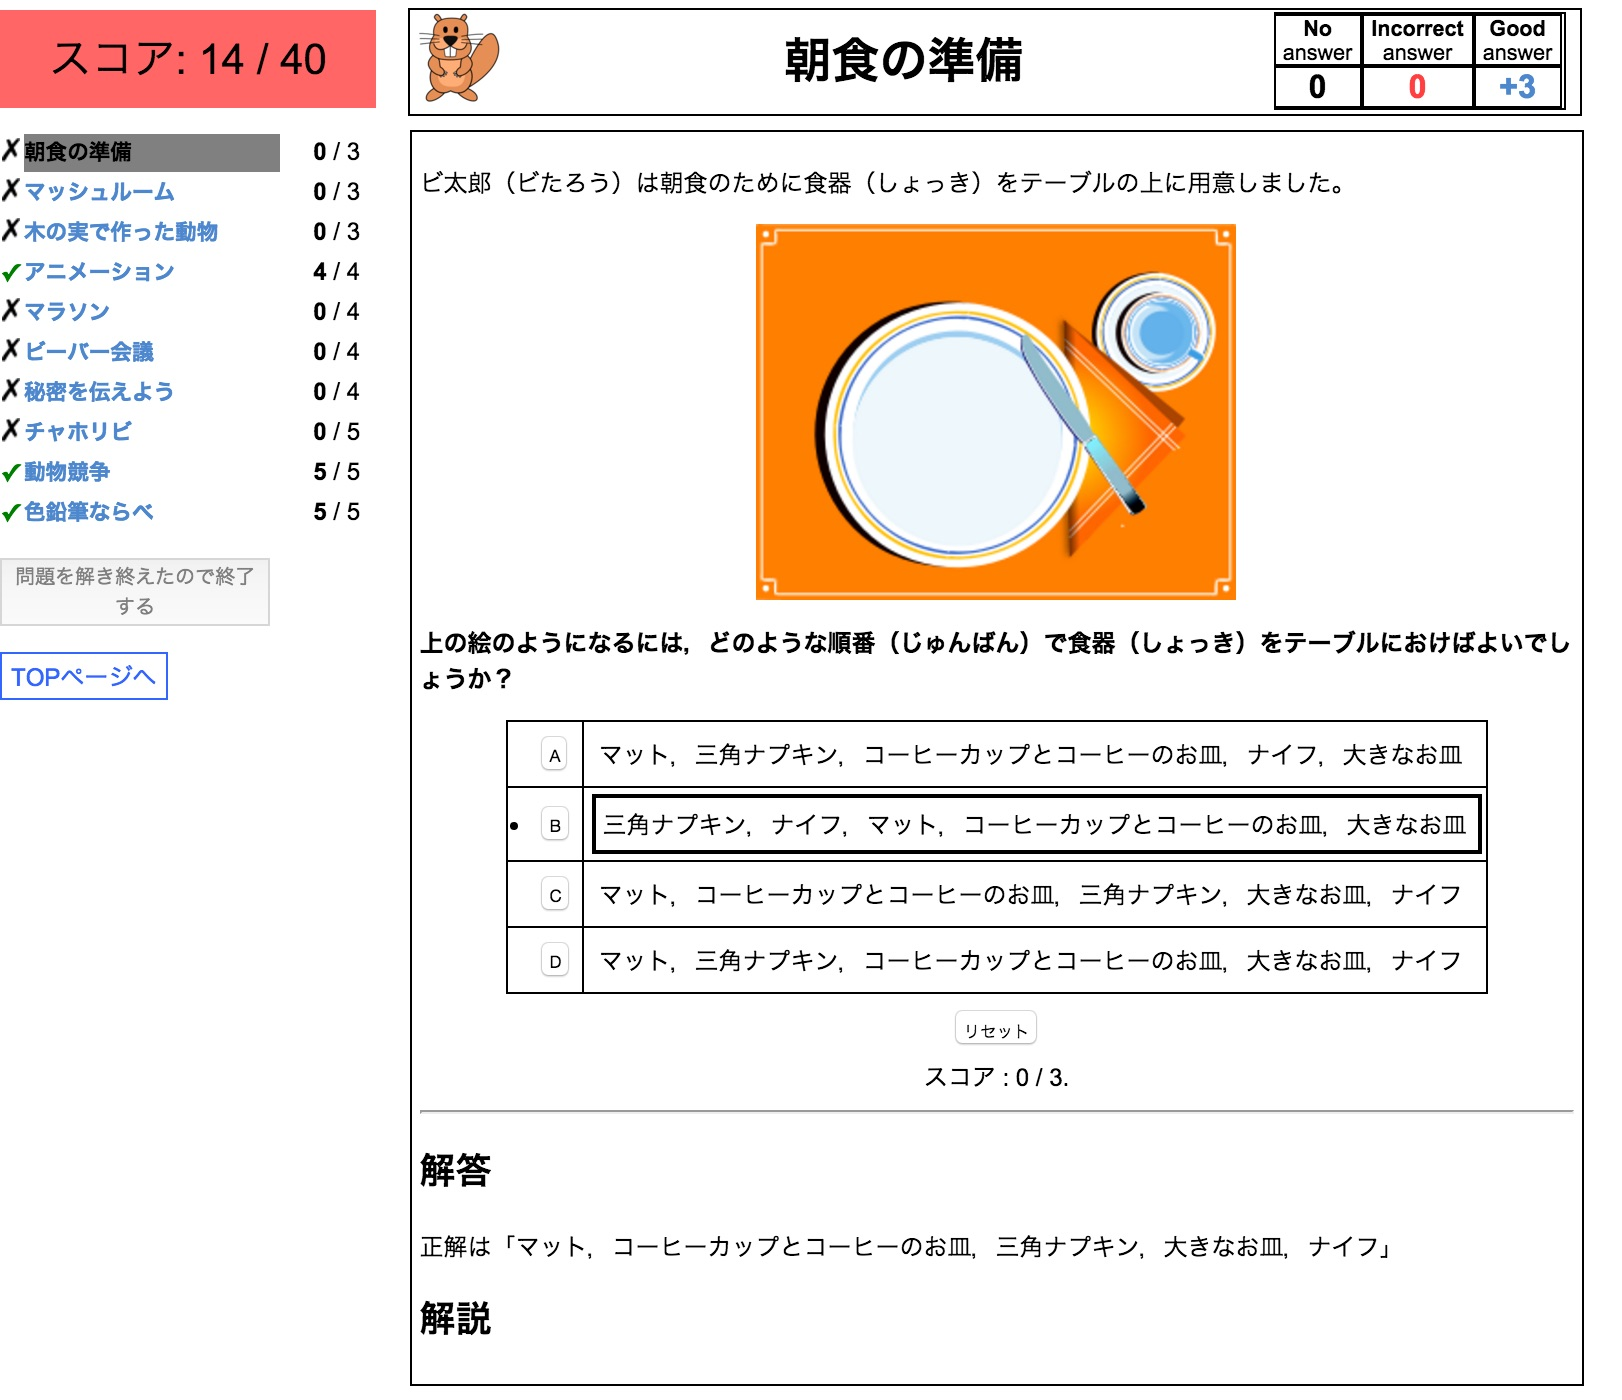
\includegraphics[bb=0 0 1622 1400,width=7.5cm]{img/new_contest_2.jpg}
}
\end{center}
\caption{新規コンテスト結果参照}\label{fig:9}
\end{figurehere}


\subsection{新規コンテスト}
管理者ページを通じてオリジナルのコンテストを作成することができる.また,個々の問題もそれぞれ新規作成することができる.
\subsubsection{新規問題の作成}
問題はWebページ上で表形式で管理でき,それぞれ問題をフォルダごとに管理することが可能となっている.また,問題の形式や答えなども表から設定することができる(図\ref{fig:10}参照).

\begin{figurehere}
\begin{center}
\fbox{
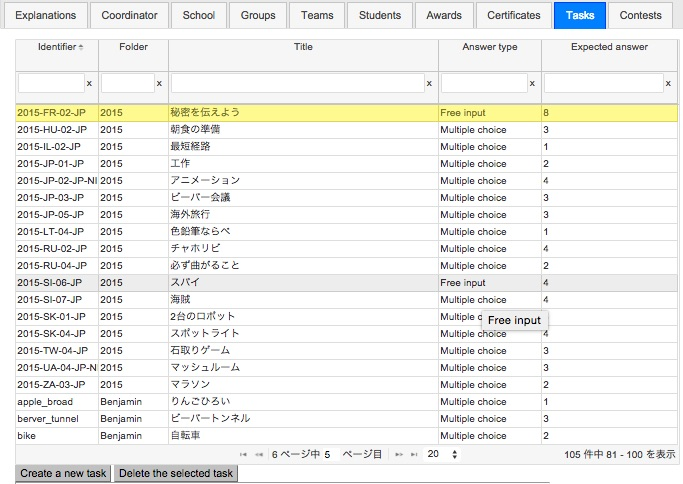
\includegraphics[bb=0 0 683 484,width=6cm]{img/bebras_task_1.jpg}
}
\end{center}
\caption{問題管理画面}\label{fig:10}
\end{figurehere}

\subsubsection{新規コンテストの作成}
コンテスト管理画面では,コンテストごとの状態を一括で管理できる.またコンテストごとの問題の管理も可能となっており,問題ごとの点数などもこの管理画面から調整することができる(図\ref{fig:11}〜\ref{fig:12}参照).

\begin{figurehere}
\begin{center}
\fbox{
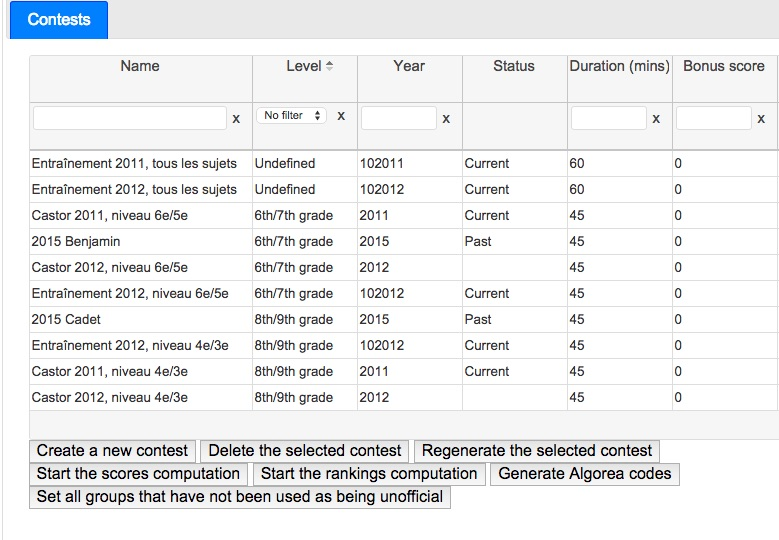
\includegraphics[bb=0 0 779 540,width=7cm]{img/create_contest_1.jpg}
}
\end{center}
\caption{コンテスト管理画面}\label{fig:11}
\end{figurehere}

\begin{figurehere}
\begin{center}
\fbox{
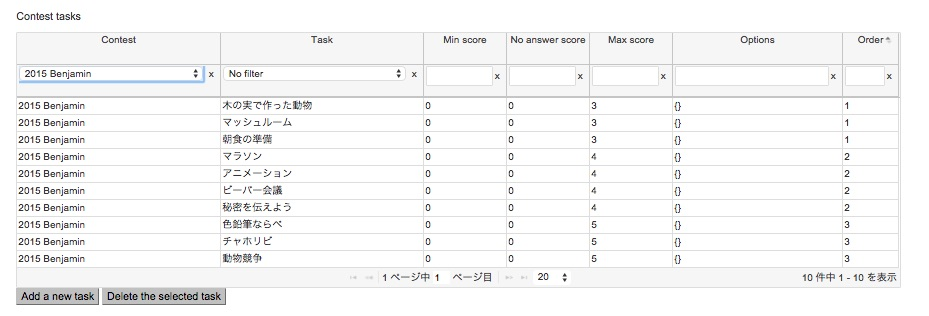
\includegraphics[bb=0 0 929 316,width=7cm]{img/create_contest_2.jpg}
}
\end{center}
\caption{コンテストごとの問題管理画面}\label{fig:12}
\end{figurehere}

\section{終わりに}
本演習では,フランスでオープンソースとして公開されているビーバーコンテストのサーバシステムを元に国内コンテストページを試作した. 本演習で対応できた問題形式は非対話型問題のみのため,対話型問題への対応は今後の課題として挙げられる.また,今年度のビーバーコンテストは11月に行われたが,試作したページの制作が間に合わず,正式なコンテストでの稼働ができなかった.そこで来年度以降は,正式なコンテストの受験ができることが望まれる.

\end{multicols}

%%%%% 参考文献 %%%%%
\begin{thebibliography}{1}

\bibitem{bebras-contest} 「ビーバーコンテスト」情報ページ.  http://bebras.eplang.jp/ , (参照 2015-12-08)
\bibitem{bebras-pdf} 谷 聖一, 兼宗 進, 井戸坂 幸男. 小中高生向け国際情報科学コンテストBebras.  http://www.ipsj.or.jp/magazine/9faeag0000005al5-att/peta55-11.pdf, (参照 2015-12-08)
\bibitem{bebras-france-platform} Bebras Platform. https://github.com/France-ioi/bebras-platform
\bibitem{git} Git  https://ja.wikipedia.org/wiki/Git
\bibitem{bower}Bower  http://bower.io/
\bibitem{composer}Composer  https://getcomposer.org/
\bibitem{dbv}dbv  http://dbv.vizuina.com/
\bibitem{i18n}i18n  https://ja.wikipedia.org/wiki/%E5%9B%BD%E9%9A%9B%E5%8C%96%E3%81%A8%E5%9C%B0%E5%9F%9F%E5%8C%96



\end{thebibliography}

\end{document} 




